\begin{figure}[b]
\centering
% Vector drawing generated by tools/figures/lookup.py; rerun it after changing the figure.
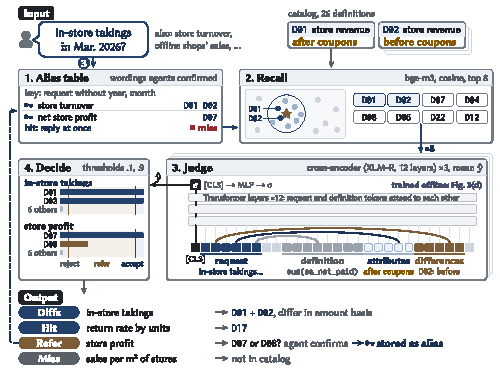
\includegraphics[width=0.90\columnwidth]{figures/lookup}%
\caption{\bt{Lightweight adaptive semantic resolution (step~3): alias lookup, dense recall, cross-encoder judging, and thresholding route a request to \code{Hit}, \code{Diffs}, \code{Refer}, or \code{Miss}; the judge's training data is built offline (Figure~\ref{fig:extraction}(d)).}{步骤~3 中的轻量级自适应语义解析：别名匹配、稠密召回、交叉编码器判别与置信度阈值将请求路由为 \code{Hit}、\code{Diffs}、\code{Refer} 或 \code{Miss}；判别器的训练数据在离线阶段构建（图~\ref{fig:extraction}(d)）。}}
\label{fig:lookup}
\Description{A flow from top to bottom, all within step 3 of Figure 2, whose badge sits on the request arrow. Input: an agent asks "in-store takings in Mar. 2026?", also worded as store turnover or offline shops' sales; the catalog of 26 definitions holds D01 store revenue after coupons and D02 store revenue before coupons. Step 1, alias table of wordings agents confirmed, keyed by the request without year and month: store turnover maps to D01 and D02, net store profit to D07; the request misses, while a hit would be answered at once. Step 2, recall with bge-m3 and cosine similarity: an embedding space where the request, a star, has D01 and D02 among the 8 points inside a circle; the candidates are D01, D02, D07, D04, D08, D06, D22, D12. Step 3, judge, a cross-encoder (XLM-R, 12 layers) run three times and averaged, once for each of the 8 candidates: the input tokens are [CLS], the request, the definition sum(ss_net_paid), its semantic attributes "after coupons", and its attribute differences "D02: before coupons"; Transformer layers let request tokens attend to definition, attribute and difference tokens; the [CLS] vector goes through an MLP and a sigmoid to score y-hat; a note says the judge was trained offline, as shown in Figure 3(d). Step 4, decide with thresholds 0.1 and 0.9: for in-store takings D01 and D02 score 1.00 and the six others 0.00, all accepted or rejected; for store profit D07 scores 1.00 and D08 0.33, in the refer zone. Output, four replies: Diffs, in-store takings gives D01 plus D02, which differ in amount basis; Hit, return rate by units gives D17; Refer, store profit gives D07 or D08 for the agent to confirm, and the confirmed wording is stored as an alias, an arrow back to step 1; Miss, sales per square meter of stores is not in the catalog.}
\end{figure}
